\documentclass[a4paper]{article}
\usepackage[top=1in,bottom=1in,left=1.25in,right=1.25in]{geometry}
\usepackage{enumerate}
\usepackage[BoldFont,SlantFont,CJKchecksingle]{xeCJK}
\usepackage{fontspec,xunicode,xltxtra}
\usepackage{amsmath}
\usepackage{graphicx}
\usepackage{float}
\usepackage{caption}
\usepackage{subfigure}
\usepackage{multirow}


%\setmainfont{Lucida Grande} % 英文衬线字体
%\setmonofont{Monaco} % 英文等宽字体
%\setsansfont{Lucida Grande} % 英文无衬线字体

\setCJKmainfont[BoldFont=Adobe Heiti Std]{Adobe Song Std}
%\setCJKmonofont{SimHei} % 设置中文等宽字体

%连字符
\defaultfontfeatures{Mapping=tex-text}
%中文断行
\XeTeXlinebreaklocale "zh"
\XeTeXlinebreakskip = 0pt plus 1pt minus 0.1pt%左右弹性间距

%%%% 缩进 %%%%
% 自动首行缩进
\usepackage{indentfirst}
% 设置首行缩进的距离
\setlength{\parindent}{2em}

\linespread{1.2} % 行距



\title{基于新浪微博中大社区的流行事件挖掘}
\author{10389003 区展明 \\ 10389079 翁镇斌 \\ 10389089 彭翼}

\begin{document}
\maketitle


\begin{abstract}在这个项目中,我们主要实现了一篇论文(见参考文献[1])提出的流行事件挖掘算法。首先,我们对微博的内容进行提取,并对一个词语(item)的生命周期进行建模。如果一个词语在给定的时间间隔中频繁出现,而在过去很少出现,我们认为它是新兴词语(emerging term)。其次,考虑到一条微博的重要性依赖于微博的作者,我们采用了PageRank算法对微博用户的权威性进行评估。最后,我们采用了Affinity Propagation[2]的聚类算法将新兴词语联系起来,挖掘出流行话题。
\end{abstract}




\section{动机}
每天生活在中大的社区中,你又是否了解过发生在你身边的时事热点?又是否清晰的知道,中大的同学都在关注些什么?我们课程设计的项目为了帮助我们了解中大人在过去的一段时间中都在新浪微博上关注些什么热点话题以及重大时事,同时,挖掘出这些流行事件产生的时间。\\
\indent 如果你有一段时间没有刷微博了,只要查看我们提取出来的流行话题,马上就可以了解新浪微博中大社区在过去一段时间内发生的热门事件,一点也不用担心自己会out了。



\section{微博内容提取}
给定一个时间间隔,我们需要在新浪微博中大社区中搜索流行的话题。假设用户设定了时间范围$r$(依赖于用户需要的检测频率),我们可以定义第$t$个时间间隔$I^t$,
\begin{align}
    I^t=<i_t,i_t+r>
\end{align}
其中,$i_t$是第$t$个时间间隔的开始时刻($i_0=0$表示第一个被考虑的时刻)。在时间间隔$I^t$中,我们提取到了词库$TW^t$,包含$n=|TW^t|$条微博。我们的目标是,将每一条微博$tw_j$抽取出特征形成一个微博向量$\vec{tw_j}$。换句话说,我们希望用一个向量$\vec{tw_j}$来代表一条微博$tw_j$。\\
\indent 首先,我们对微博做分词处理,使用了基于Python的jieba分词。虽然[1]中提到他们并没有使用stop words,但我们在实验的过程中发现,有些没有意义的词语,比如“了”,会成为被检测到的新兴词语,而且,在根据新兴词语构建流行话题的这一步,我们也没有完全采用[1]提出的方法。因此,我们启用了一个stop words列表,列表中的词语一部分来源于网上搜集到的数据,另外一部分是新浪微博中的表情。另外,我们将jieba分词得到的单个字也过滤掉,因为单字的词通常情况下都没有太多的信息。\\
\indent 接着,我们对每一条微博进行分词,可以得到一个词汇表(vocabulary)。计算第$j$条微博的词汇表中的第$x$个词语的权重$w_{j,x}$,采用augmented normalized term frequency的方法,
\begin{align}
    w_{j,x}=0.5+0.5 \cdot \frac{tf_{j,x}} {tf_{j}^{max}}
\end{align}
其中,$tf_{j,x}$是第$j$条微博的词汇表中的第$x$个词语在这条微博中出现的次数,$tf_{j}^{max}$表示第$j$条微博的词汇表中词语出现的最大次数。因而,对于每一条微博$tw_j$,表示该微博的向量可以定义为
\begin{align}
    \vec{tw_j}=\{w_{j,1}, w_{j,2}, \cdots, w_{j,v}\}
\end{align}
其中,$v$是词汇表的大小(size)。\\
\indent 经过这一个步骤后,在给定的时间间隔中,每条微博所表示的信息已经被正规化(formalize)为一个带有权重的微博向量。



\section{评估用户权威性}
在新浪微博上,加v的大户一条微博可以轻松地获得上万的转发量。虽然微博本身的文本内容已经包含了我们要检测的流行事件的绝大部分信息,但是,一条微博是否是有影响力的微博用户发出的,依然对这条微博所描述的事件能否成为流行事件有巨大的影响。因此,我们希望对新浪微博中大社区的用户的权威性做评估。\\
\indent 在新浪微博中,我们可以定义一个社会网络关系图$G(U,F)$,$U$是用户集合,$F$是有向边的集合,因而,给定两个微博用户$u_i$和$u_j$,存在一条从节点$u_i$指向$u_j$的边$<u_i,u_j>$当且仅当$u_i$是$u_j$的粉丝。这样定义的社会网络关系图和互联网的网页图谱异曲同工,因此 ,我们可以用经典的PageRank算法,计算出每个用户在给定的社会网络关系图中的重要性,即用户权威性。\\
\indent 根据PageRank算法和我们获得的新浪微博中大社区的用户关注列表,可以初始化矩阵$M'$。通过分析矩阵$M'$,我们可以找到在这个网络关系图中的dead end。如果该图谱中的一个用户$u_i$没有关注该图谱中的任何一个用户,我们称用户$u_i$是一个dead end。矩阵$M'$中用户$u_i$所在的列全为0,根据线性代数的知识,dead end的存在会使得矩阵迭代无法收敛。因此,我们需要先去除dead end,处理之后的矩阵记为$M$。\\
\indent 现在我们可以迭代计算用户的权威指数了。每个用户的权威指数组成的向量$\vec{v}$可由以下公式迭代得出,
\begin{align}
    \vec{v'}=\beta M\vec{v}+(1-\beta) \frac{\vec{e}} {n}
\end{align}
其中,$n$是图谱中节点的总数,即社区中微博用户的数量(去除dead end之后),$\vec{e}$是单位向量,$\beta$是一个跳转概率(teleport probability),在项目中我们设定为0.85,$\vec{v}$的初始值为$\frac{\vec{e}} {n}$,$\vec{v'}$是新一轮迭代得到的用户权威指数向量。\\
\indent 由于我们所考虑的社会关系图比较小,矩阵$M$可以放在内存中,因此,算法并不复杂。在项目中,我们只需迭代20次就发现$\vec{v}$基本收敛了。迭代结束后,我们可以根据指向dead end的节点的权威指数反向推出dead end的权威指数。



\section{新兴词语的挖掘}
一个新兴词语通常可以被认为是指向最近发生的流行事件的语义单元。我们寻找新兴词语目标的实现依赖于对微博和作者的精确建模。在[1]中提出了两个概念,词语营养和词语能量,基于统计对词语的生命周期进行定量和定性的分析。
\subsection{词语营养(Content Nutrition)}
对于在语料库中的每个词语,我们可以将其类比成为一个活生生的生物,其生命周期可以这样定义:当有充足的食物营养(包含该term的微博)供应,该term的生命周期得到了延续;但是,当食物营养供应不足时,该term的生命周期将会减少甚至死亡。\\
\indent 根据这个原理,我们可以定义一个词语的nutrition如下:当一个词语的nutrition值越高,代表着这个词语在相应的时间段中越热。当nutrition值很低,表明该词语在相应时间内很少出现。因此,在时间间隔$I^t$中,对于$k\in K^t$和$TW_k^t\in TW^t$,$TW_k^t$表示微博库中包含词语$k$的微博,我们可以计算词语$k$的nutrition值,
\begin{align}
    nutr_k^t=\sum_{tw_j\in TW_k^t} w_{k,j}*auth(user(tw_j))
\end{align}
其中,$w_{k,j}$表示词语$k$在微博向量$\vec{tw_j}$中的权重。$user(tw_j)$返回发表微博$tw_j$的用户$u$,$auth(u)$表示微博用户$u$的权威指数。我们可以看出,词语$k$的nutrition值的计算,结合了它在微博库中的热度以及发表这些微博的用户的权威性。

\subsection{词语能量(Content Energy)}
通过上一步计算每个词语的nutrition值后,我们可以得出哪些词语在被考虑的时间段内被引用的次数较多。但是,在本项目中,我们要寻找的是在某个时间段内的热门事件或新兴事件,而一个词语是新兴词语的定义如下:\\
\indent 一个词语如果被定义为emergent,那么它应该是在指定的时间段内热度(nutrition值)很高,但是在过去的一段时间内热度较低。\\
\indent 我们不需要考虑所有的历史情况,因为一个词语变成emergent后,一段时间后,也会有可能再度成为emergent词语。例如2011年6月11日,因为郭美美的炫富事件,“红十字会”成为当时的热门词语;而在2013年4月末,雅安地震后大家对红十字会的冷漠,再一次让词语“红十字会”成为热门词语。但是,总的来说,如果两个词语在短时间内nutrition值非常接近,那么,这两个词语代表的很可能是同一个事件。在这种情况下,根据我们的定义,即使这个词语的热度(nutrition值)很高,它仍然不能被认为是新兴词语,因为新兴词语的定义还要求它在过去的一段时间热度较低。因此,我们有必要引入词语能量这一概念来检测新兴词语。\\
\indent 我们必须注意到,用户指定的时间间隔$I^t$的大小对检测到的新兴词语的类型有很大影响。例如,假设某些词语只在一个用户的微博中出现过,如果我们考虑一个较短的时间间隔(比如一天),系统检测到的新兴词语大多会是关于日常生活的,而如果我们考虑一个较长的时间间隔,系统检测到的新兴词语大多会是关于那些日常生活中很少出现的,比如意外事件。因此,我们引入了一个参数$s$,满足$0<s<t$,它限制了系统在对词语的生命周期进行建模的过程中需要考虑的过去的时间片(time slots)的个数。\\
\indent 根据上述的理论基础,给定词语$k$,在时间间隔$I^t$中,我们可以定义一个词语的energy值,
\begin{align}
    energy_k^t=\sum_{x=t-s}^{t} \frac{(nutr_k^t)^2-(nutr_k^x)^2} {t-x}
\end{align}
其中,$nutr_k^x$表示在时间间隔$I^x$中词语$k$的nutrition值。词语的energy值越高,代表词语在指定的时间段内爆发性和热度越强。



\section{从新兴词语(term)到新兴话题(topic)}
新兴词语term是事件的重要表征,但term只是单个词语,其对事件的表达能力有限。即使是表征性较强的词语,如在2013年4月20日(这天发生了雅安地震)爆发的新兴词语“地震”。见到这个词语,我们很容易联想起来的是雅安地震的消息报道以及救援工作的进展。但是,在地震发生后的7到8天,我们再次检测到新兴词语“地震”,但此时“地震”指向的事件与之前的相比已经有了很大的不同,它更多的是关于灾后救助,爱心捐款的消息。由此看来,term对事件的表达能力不足。\\
\indent 因此,term聚合的目的是将描述同一个事件的term聚到一起,组成一个新的topic,增加其对事件的表达能力,提高用户体验。换句话说,我们用一个事件的关键词(term)集合来表征一个事件。

\subsection{关联数组}
在我们的项目中,我们定义一个新兴话题是一个新兴词语的集合。对于每一个词语$k\in EK^t$,可以定义一个相关性向量$\vec{cv_k^t}$,表示第$k$个词语和其他词语在给定时间间隔中的相关性。为了度量第$k$个词语和第$z$个词语之间的相关度,我们认为微博库中同时包含这两个词语的微博是支持这种关系的正面证据(positive evidence),而那些只包含一个词语的微博是支持这种关系的负面证据(negative evidence)。因此,在时间间隔$I^t$中,第$k$个词语和第$z$个词语的相关性权重$c_{k,z}^t$,基于probabilistic feedback mechanism可以定义如下,
\begin{align}
    c_{k,z}^t=log \frac{ {r_{k,z}} / (R_k-r_{k,z}) } { (n_z-r_{k,z}) / {N-n_z-R_k+r_{k,z}} } \times |\frac {r_{k,z}} {R_k} - \frac {n_z-r_{k,z}} {N-R_k}|
\end{align}
其中,
\begin{itemize}
    \item $r_{k,z}$表示在$TW_k^t$中同时包含第$k$个词语和第$z$个词语的微博总数
    \item $n_z$表示在微博库中包含第$z$个词语的微博总数,它等于$|TW_z^t|$
    \item $R_k$表示在微博库中包含第$k$个词语的微博总数,它等于$|TW_k^t|$
    \item $N$是微博的总数
\end{itemize}
因而,给定第$k$个词语,在时间间隔$I^t$中,它与其他$v$个词语的相关度可由相关性向量$\vec{cv_k^t}$表示,
\begin{align}
    \vec{cv_k^t}=<c_{k,1}, c_{k,2}, \cdots, c_{k,v}>
\end{align}
其中,$v=|K^t|$。

\subsection{Affinity Propagation聚类}
将2.1得到的关联数组组成矩阵$S$,其中,$S(i,j)$表示词语$i$,$j$之间的相似性。将矩阵$S$作为聚类算法的输入,对term进行聚类,其聚类结果就是相应的topic。\\
\indent 传统的聚类算法如K-Means,Hierarchical cluster等聚类算法,都直接或间接的要事先设置好分类的数目,而由于在项目中,无法得知热门的terms中,到底包含了多少个topic,因此效果均不佳。\\
\indent 此外,如K-means算法中,起始时候需要随机的选择若干exemplars作为分类点的中心,此后通过不断的迭代调整cluster的中心点以缩小误差。在此类算法中,起始数据点的选择对聚类结果有比较大的影响,因此,聚类的效果并不稳定。尽管通过更换初始选择,运行算法多次从中选择效果最好的聚类结果可以从一定程度上提高聚类效果,但是这需要在cluster较少,并且初始选择的种子比较接近优良解(good solution)的条件下,才会有较大的提升。\\
\indent 而Affinity Propagation算法在起始时,把所有的数据节点都视为exemplars(一个聚类中最具代表性的点在AP算法中叫做exemplar),并将每个term看成关系图中的一个节点,通过节点之间不断的消息传递,其中,节点之间传递的消息的强弱反映出当前节点选择某个节点作为exemplar以及某个节点认为自己适合当exemplar的置信度。据此,通过消息的迭代逐步生成图中对应的聚类簇。\\
\indent Affinity Propagation算法接受两两数据节点之间的相似性矩阵作为输入。在项目中,我们的输入是每个term的关联数组所组成的相似性矩阵$S$,其中,$S(i,j)$表示数据节点$i$,$j$之间的相似性。$S(i,j)$的值越大,$i$,$j$相似度越高。注意,矩阵S并非一定是对称矩阵,也就是说$i$,$j$的相似性和$j$,$i$的相似性不一定相同。\\
\indent 相比于K-means等聚类算法要求直接指定cluster的数量, AP算法接受一组输入参数preferences:$[s(k,k)...]$,其中,$s(k,k)$越大,在后续的迭代中, k被选择作为exemplar的可能性越大。当每个$s(k,k)$都很大的时候, 每个点都以自我为中心, 迭代结果将是所有点各自成为一个cluster。因此,参数preferences也将直接影响到结果中cluster的数目。在本项目中,preference的值被预设为$Median(s(i,k'),k'!=i)$。\\
\indent AP算法中,在数据点之间传递的消息主要有两种:
\begin{itemize}
	\item \textbf{responsibility} $r(i,k)$,从节点$i$发送到候选exemplar节点$k$上,代表着节点$k$能够胜任节点$i$的exemplar的置信度,反映节点$k$作为exemplar的能力。
	\item \textbf{avaliability} $a(i,k)$,从候选exemplar节点$k$发送到数据节点$i$上,反映节点$i$会选择节点$k$作为它的exemplar的置信度,反映了节点$i$对节点$k$的支持。
\end{itemize}
其中,算法起始时设置所有的$a(i,k)=0$,responsibility消息的计算方法如下:
\begin{align}
r(i,k)\leftarrow s(i,k) - \max_{k'\neq k} \left\{ a(i,k') + s(i,k') \right\}
\end{align}
$r(i,k)$可以理解为,节点$k$本身有多少能力去胜任节点$i$的 exemplar,其中,$k$与其他节点竞争的结果(体现在上述公式中)可以有效的反映出$k$点的竞争力。\\
\indent 特别地,当$i=k$时,
\begin{align}
r(k,k)\leftarrow s(k,k) - \max_{k'\neq k} \left\{ a(k,k') + s(k,k') \right\}
\end{align}
在这里,$r(k,k)$反映出$k$本身作为exemplar的置信度。其中$s(k,k)$即为上述所说$k$点的preferences,可以看出,$s(k,k)$越大,$r(k,k)$越大。\\
\indent 而avaliability消息的计算方式如下,
\begin{align}
a(i,k)\leftarrow \min \left\{ 0, r(k,k) + \sum_{i'\notin \left\{ i,k \right\}} \max \left\{ 0, r(i',k) \right\} \right\}
\end{align}
其中,$a(i,k)$反映出节点$i$选择节点$k$作为它的exemplar的置信度。从公式中可以直观看出,节点$i$对节点$k$的支持,来源于以下两部分,
\begin{enumerate}
    \item $r(k,k)$,$k$想成为exemplar的意愿的强烈程度。
    \item $\sum_{i'\notin \left\{ i,k \right\}} \max \left\{ 0, r(i',k) \right\}$,$k$有多适合当任其他点的exemplar的能力体现。
\end{enumerate}
注意到在第2项中,只有大于0的$r(i',k)$被加上,而小于0的则被忽略。因为在这里,只需要考虑$k$点有多适合当其他点的exemplars,而不需要考虑$k$点有多不适合当其他点的exemplar,即只需要考虑$k$对它的簇类的统治能力。\\
\indent 此外,上述公式中,当$r(k,k)$为负时,意味着节点$k$更偏向于选择其他节点作为exemplar,而不是自己当任exemplar。但此时,可能会存在$r(k,k) + \sum_{i'\notin \left\{ i,k \right\}} \max \left\{ 0, r(i',k) \right\} > 0$的情况,从而导致$a(i,k)$增长(因为起始$a(i,k)$为0)。那么此时应该遏制这种趋势,因此应该将$a(i,k)$的范围控制在0以下。\\
\indent Affinity Propagation算法的终止方式有2种,
\begin{enumerate}
    \item 达到预定的迭代次数
    \item 传递的消息的变化量低于某一个阈值
\end{enumerate}

总的来说,Affinity Propagation算法具体有以下步骤,
\begin{enumerate}
    \item 根据avaliability消息的值,更新所有的responsibility消息的值。
    \item 根据新的responsibility消息的值,更新所有的avaliability消息的值。
    \item 结合消息responsibility和消息avaliability,决定当前迭代结果中的exemplar以及哪些点属于哪个exemplar,并确定算法是否应该结束。
\end{enumerate}



\section{实验环境}
\begin{enumerate}
    \item Operating system: Linux(Ubuntu, with 3.0+ kernels)
    \item Language: Python 2.7
    \item Editor: VIM
    \item Documentation: \LaTeX
\end{enumerate}



\section{数据获取及处理}
\subsection{用户群体}
本次项目的用户群体为8,000名的中山大学微博用户。我们的做法是,选取中大多个学院的几个种子用户,根据种子用户的关注列表,一层一层往外搜索,直到找到8,000名中山大学微博用户。如果获取数据能够更方便一些,我们的机器更好一些,也可以将新浪微博的所有中大微博用户都搜集到。
\subsubsection{中大身份的判定}
用户群体的爬取主要通过网页爬虫爬取用户,并且通过用户个人信息中“毕业于”一栏所填的大学来判定用户是否为中大人。
\subsubsection{判定方法的优劣}
\paragraph{优点}数据纯度都要比传统的聚类以发现社区群体要高, 一方面大大避免的僵尸粉/广告微博用户的出现(这类用户很少填写自己的毕业学校)。
\paragraph{缺点}效率低下,爬虫爬取信息耗费大量时间, 遗漏了某些没有填写毕业学校的中山大学的微博用户。

\subsection{用户关系图谱的建立}
\begin{enumerate}
    \item 通过新浪API获取每个用户的好友关注列表。
    \item 筛选用户好友关注列表,只保存存在于用户群体的用户。
    \item 根据微博用户相互关注的情况,建立用户关系图谱。
\end{enumerate}

\subsection{微博数据}
本次项目中,我们爬取了8,000名用户最近发布的400条个人信息,共2,460,342条微博作为实验数据。其中,在2013年4月至2013年5月,平均每天的微博数量有8,200多条。Figure 1显示了我们获取到的新浪微博中大社区2013年4月1日至2013年5月1日每天发布的微博数量。需要特别说明的是,在挖掘流行事件的过程中,我们的时间间隔(time interval)都设置为1天。
\begin{figure}[htbp]
\centering
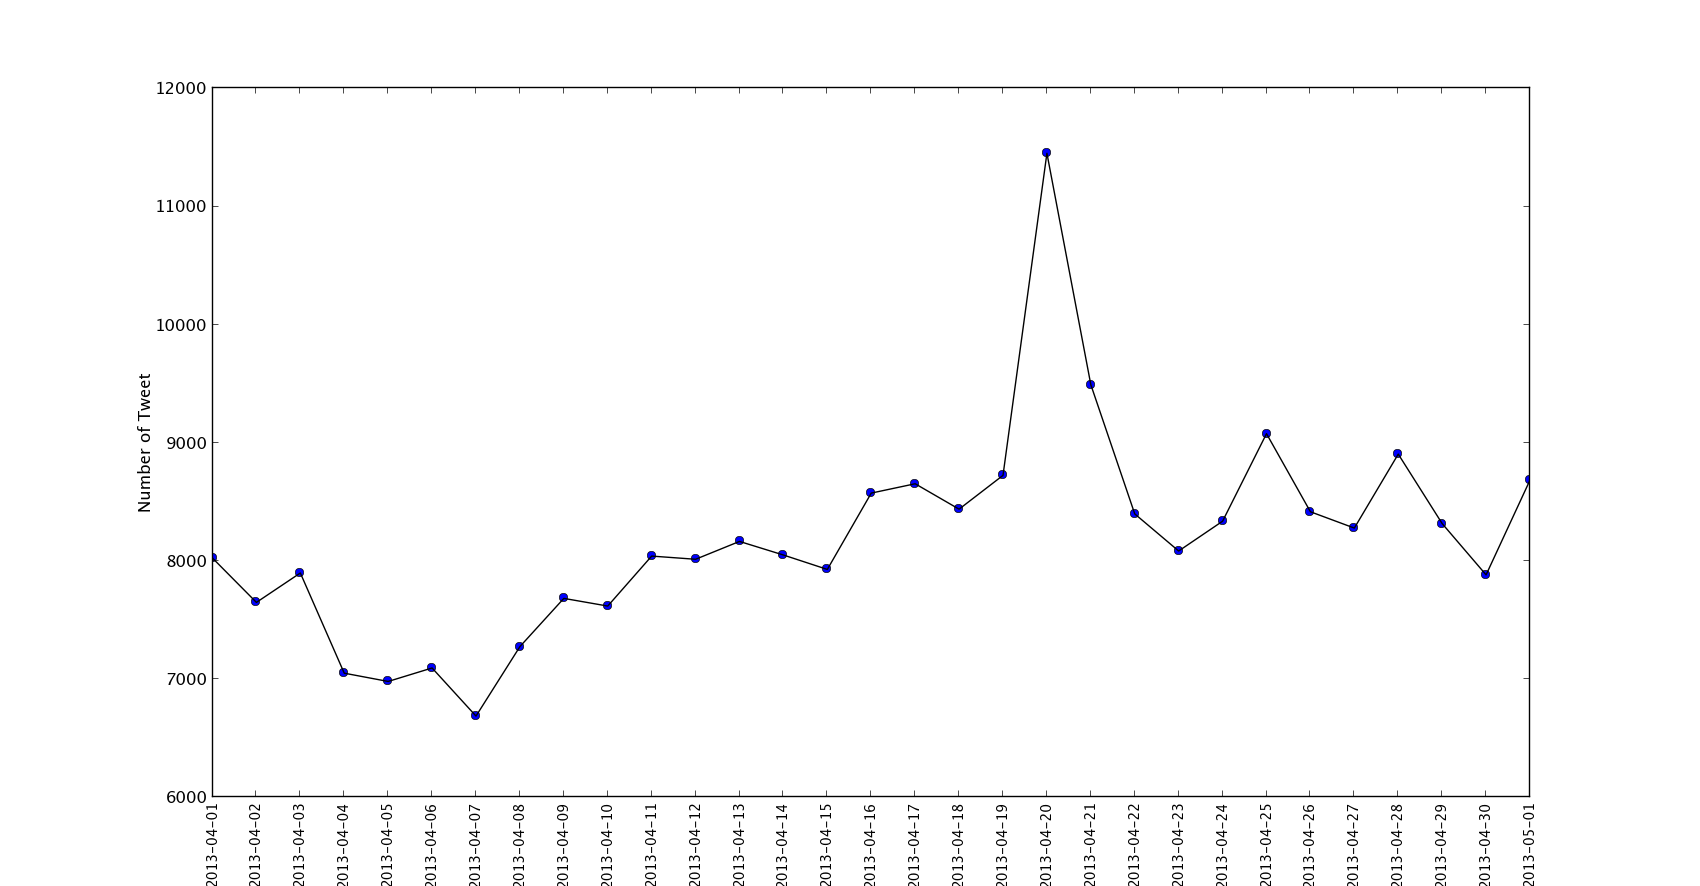
\includegraphics[width=5.5in]{num_of_weibo_between_April_May.png}
\caption{2013年4月1日至2013年5月1日每天发布的微博数量}
\label{fig:1}
\end{figure}



\section{测试分析}
我们采用了PageRank算法对抓取到的8,000名微博用户的权威性进行评估,Figure 2是用户权威性排名前50名的列表。从列表中可以看出,排名较前的都是在新浪微博中大社区较有影响力的微博用户。比如,中大Din,因为经常转发同学们丢失物品的微博,以及拥有一个可以帮助分析微博的筛选器,在社区中有很高的人气,因此,用户权威性排行榜上名列第一。在列表上排名前十中有许多中大的老师,比如朱孔军(校党委副书记),竹帛斋主(图书馆馆长程焕文),中大软件学院团委廖喜扬和中大软件学院张硕辰。这些微博用户上榜,主要是因为他们在学生中有较高的知名度。在榜单中,上榜的微博用户还包括一些交际比较广的人,比如活跃于学生会或者团委的同学。另外,一些组织或者社团也拥有较高的权威性,例如中山大学逸仙时报,逸仙周刊和中大传播与设计学院。
\begin{figure}[H]
\centering
\subfigure[用户权威性排名1到25名列表]{
\label{Fig.sub.1}
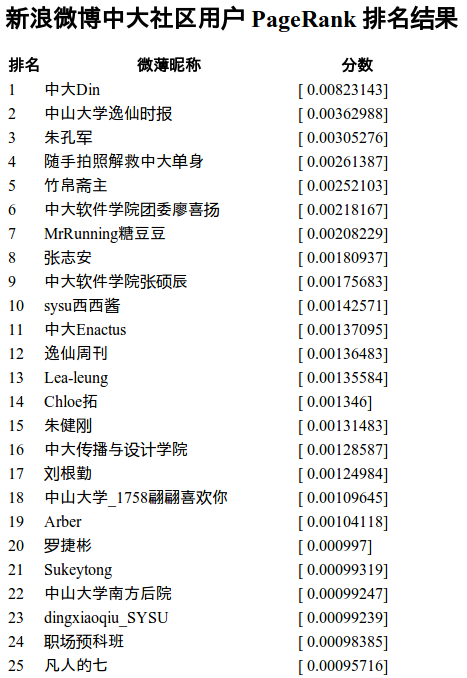
\includegraphics[width=0.45\textwidth]{pagerank1.png}
}
\subfigure[用户权威性排名26到50名列表]{
\label{Fig.sub.2}
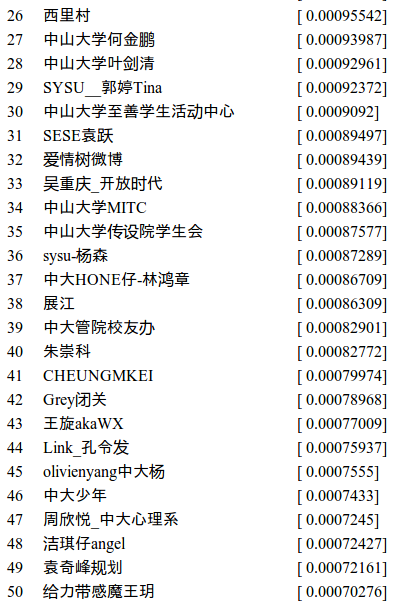
\includegraphics[width=0.45\textwidth]{pagerank2.png}
}
\caption{用户权威性排名前50名列表}
\label{fig:2}
\end{figure}

\indent 为了找到新兴词语,我们使用了词语营养(Content Nutrition)和词语能量(Content Energy)两个概念。Figure 3显示了词语“同学”的nutrition值和energy值走势图。由于“同学”在新浪中大社区的微博中经常出现,因此我们可以从走势图发现,无论是nutrition值还是energy值,其走势都是不断地起伏,并不存在某些非常显著的爆发点。所以,“同学”这样的词语,在社区中一般不会成为新兴词语。另外,一些日常用语,也不太可能成为新兴词语,一个典型的例子是时间描述词,例如“早上”。Figure 4显示了词语“早上”的nutrition值和energy值走势图,这个走势图比词语“同学”的更趋平缓。
\begin{figure}[H]
\centering
\subfigure[词语“同学”的nutrition值走势图]{
\label{Fig.sub.1}
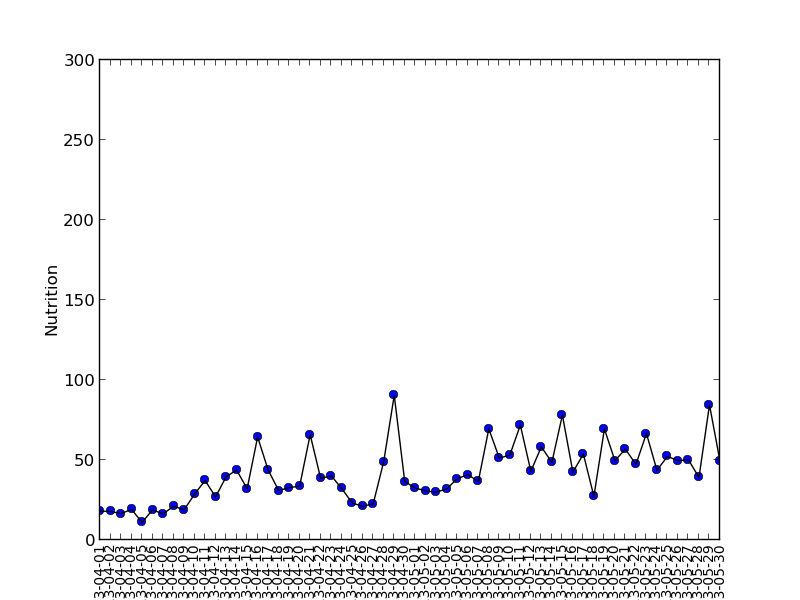
\includegraphics[width=0.45\textwidth]{同学_nutrition.png}
}
\subfigure[词语“同学”的energy值走势图]{
\label{Fig.sub.2}
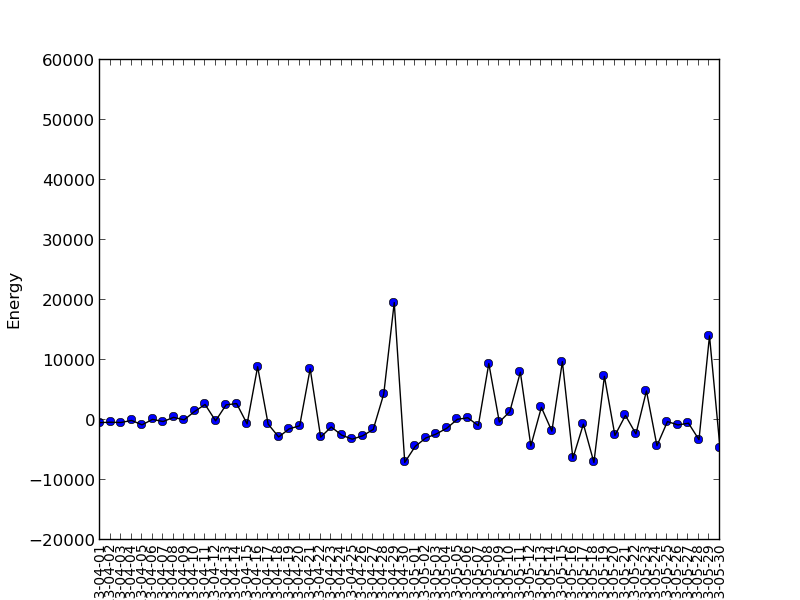
\includegraphics[width=0.45\textwidth]{同学_energy.png}
}
\caption{词语“同学”的nutrition值和energy值走势图}
\label{fig:3}
\end{figure}

\begin{figure}[H]
\centering
\subfigure[词语“早上”的nutrition值走势图]{
\label{Fig.sub.1}
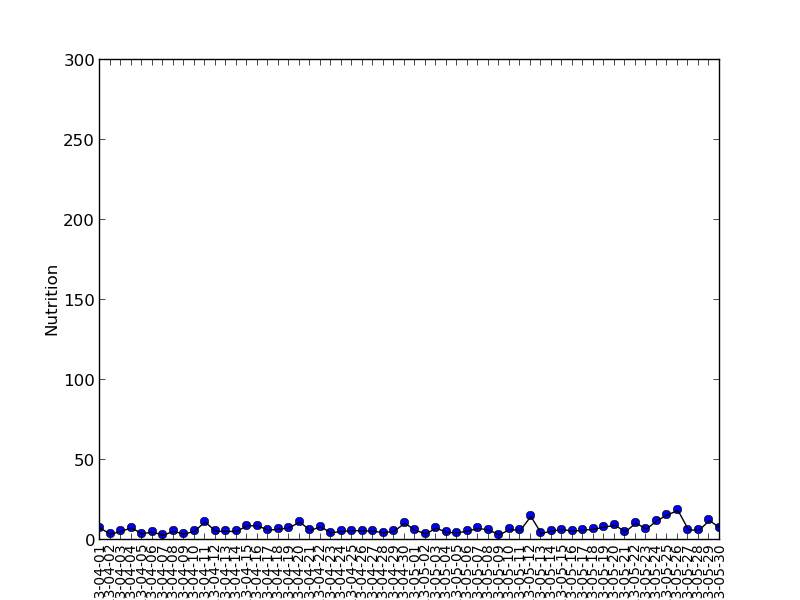
\includegraphics[width=0.45\textwidth]{早上_nutrition.png}
}
\subfigure[词语“早上”的energy值走势图]{
\label{Fig.sub.2}
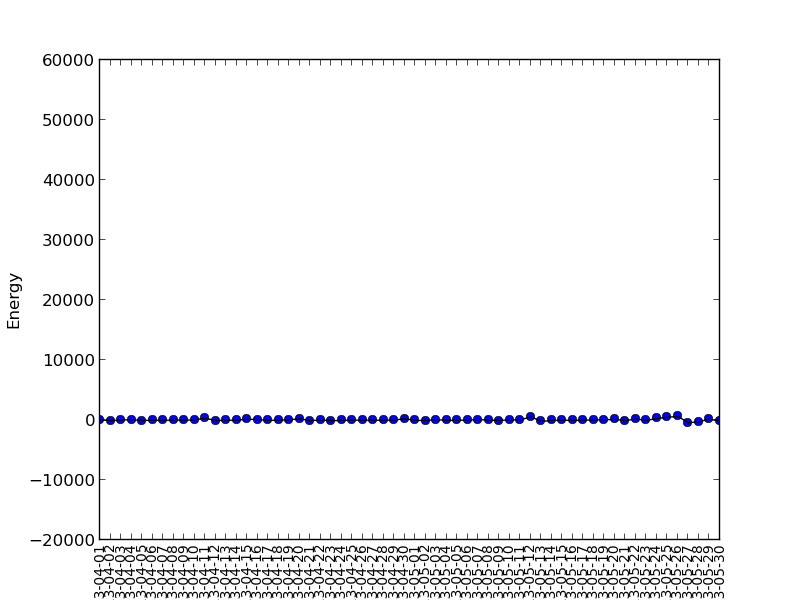
\includegraphics[width=0.45\textwidth]{早上_energy.png}
}
\caption{词语“早上”的nutrition值和energy值走势图}
\label{fig:4}
\end{figure}


\indent 现在,我们来看一些标志性的流行事件。2013年4月20日发生的雅安地震,牵动着无数中国人的心,同时,在新浪微博中大社区,也迅速成为热点话题。Figure 5显示了词语“雅安”的nutrition值和energy值走势图。在雅安地震发生之前,中大社区的微博中几乎不会提到雅安。在雅安地震发生之后,从雅安的nutrition值走势图中可以看出,词语“雅安”的热度迅速攀升,成为中大社区的热门词语。由于之前一段时间,“雅安”的热度基本为0,因此,“雅安”符合新兴词语的定义,成为被系统检测出来的新兴词语。从词语“雅安”的energy值走势图中可以发现,雅安地震发生两天后,“雅安”的energy值突然变得非常低,这是因为energy值的计算跟前一段时间是有关的。在地震发生的前两天,雅安的nutrition值非常高,到了第三天,nutrition值相对降低,因此,当天“雅安”的energy值就非常低了。
\begin{figure}[H]
\centering
\subfigure[词语“雅安”的nutrition值走势图]{
\label{Fig.sub.1}
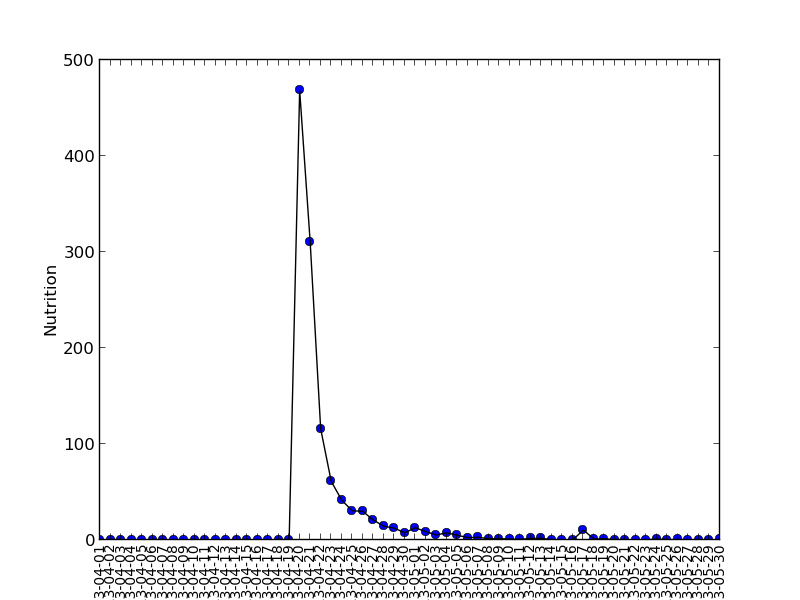
\includegraphics[width=0.45\textwidth]{雅安_nutrition.png}
}
\subfigure[词语“雅安”的energy值走势图]{
\label{Fig.sub.2}
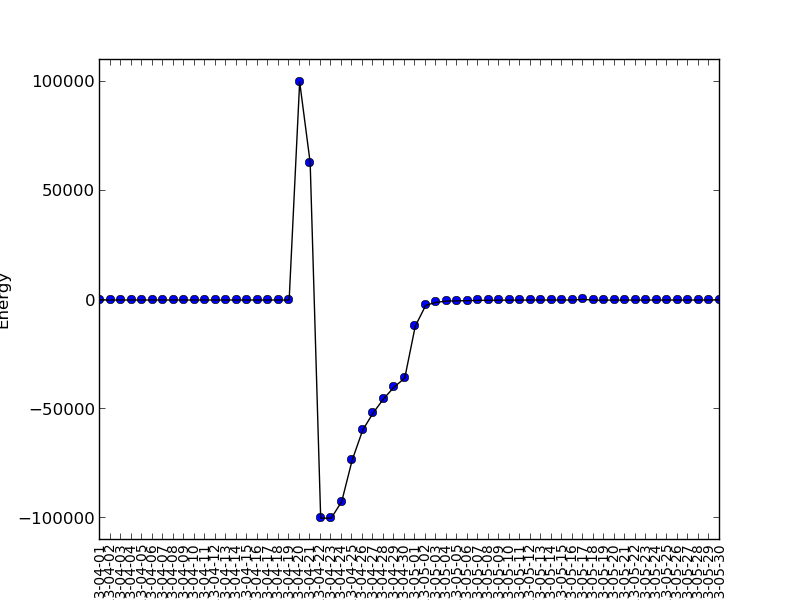
\includegraphics[width=0.45\textwidth]{雅安_energy.png}
}
\caption{词语“雅安”的nutrition值和energy值走势图}
\label{fig:5}
\end{figure}

\indent 我们的系统,不仅能挖掘到全国性的热点事件,更有意思的是它能够对社区性的热点事件进行检测。一年一度的维纳斯歌手大赛是中大的一大盛事,在维纳斯歌手赛期间,社区中关于维纳斯的讨论也非常热。Figure 6显示了词语“维纳斯”的nutrition值和energy值走势图。这两幅走势图都有两个主要的峰值,即2013年5月5日和5月11日,分别对应于两个比较热门的事件,维纳斯歌手大赛的四校区决赛和微博上转发次数很多的明星祝福“维纳斯”的视频。
\begin{figure}[H]
\centering
\subfigure[词语“维纳斯”的nutrition值走势图]{
\label{Fig.sub.1}
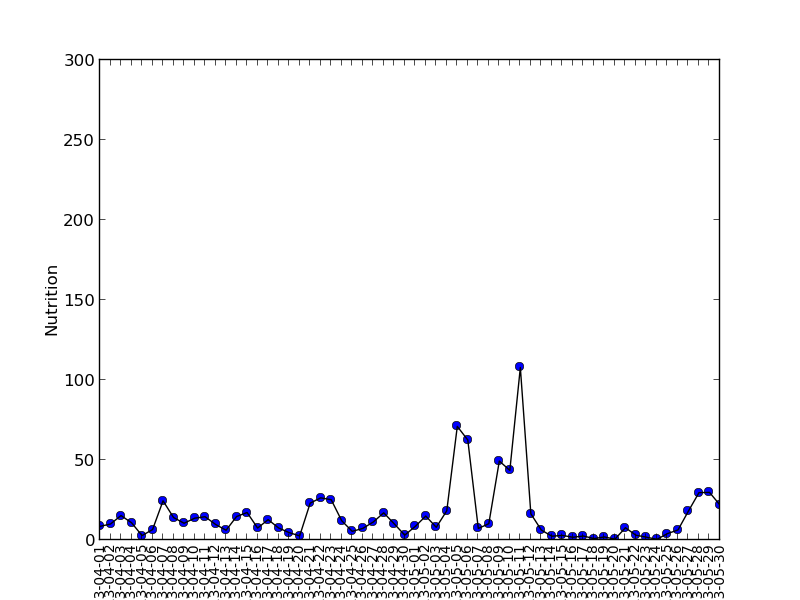
\includegraphics[width=0.45\textwidth]{维纳斯_nutrition.png}
}
\subfigure[词语“维纳斯”的energy值走势图]{
\label{Fig.sub.2}
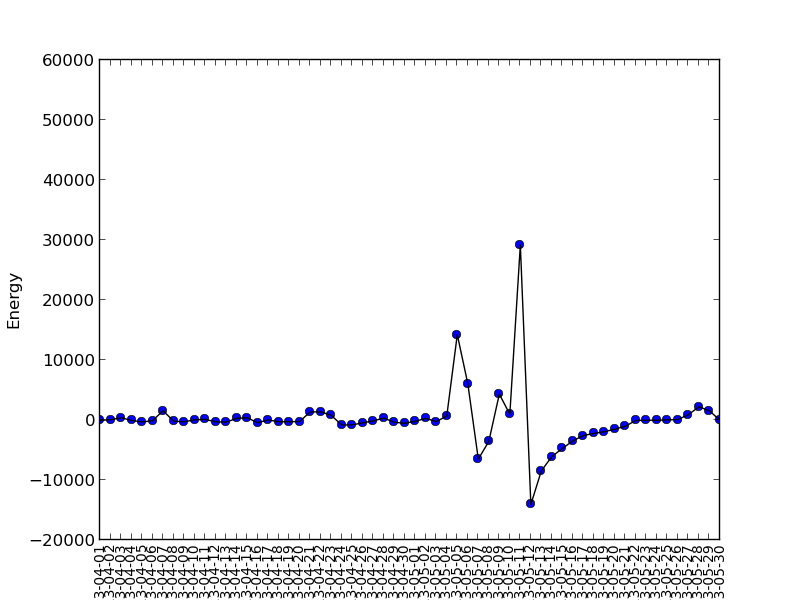
\includegraphics[width=0.45\textwidth]{维纳斯_energy.png}
}
\caption{词语“维纳斯”的nutrition值和energy值走势图}
\label{fig:6}
\end{figure}

\indent 同样是中大的热点事件,首届中大自由格斗赛的关键词“格斗”,也作为新兴词语被检测出来。Figure 7显示了词语“格斗”的nutrition值和energy值走势图。2013年4月27日,词语“格斗”的nutrition值很高,因为那时候恰好是格斗赛的报名日期。5月11日,格斗赛的现场视频在微博上出现,因此当天词语“格斗”的energy值很高,“格斗”成为新兴词语。
\begin{figure}[H]
\centering
\subfigure[词语“格斗”的nutrition值走势图]{
\label{Fig.sub.1}
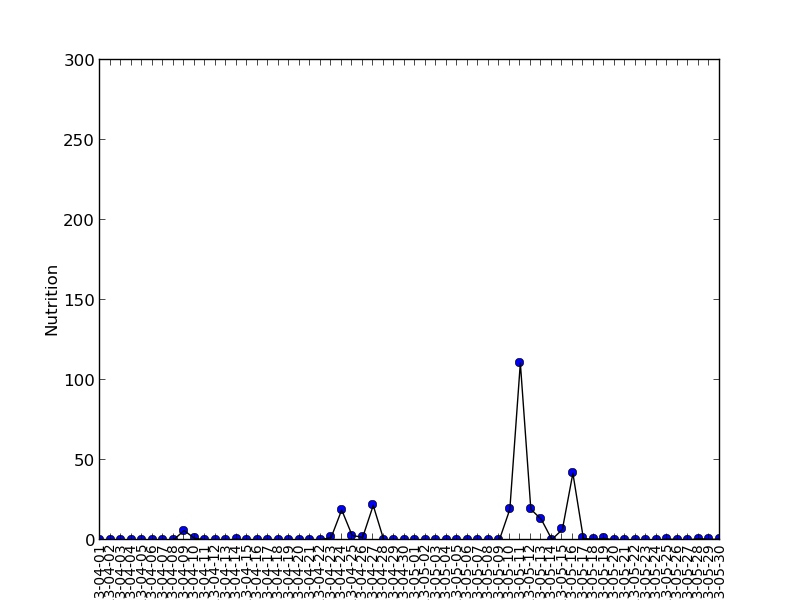
\includegraphics[width=0.45\textwidth]{格斗_nutrition.png}
}
\subfigure[词语“格斗”的energy值走势图]{
\label{Fig.sub.2}
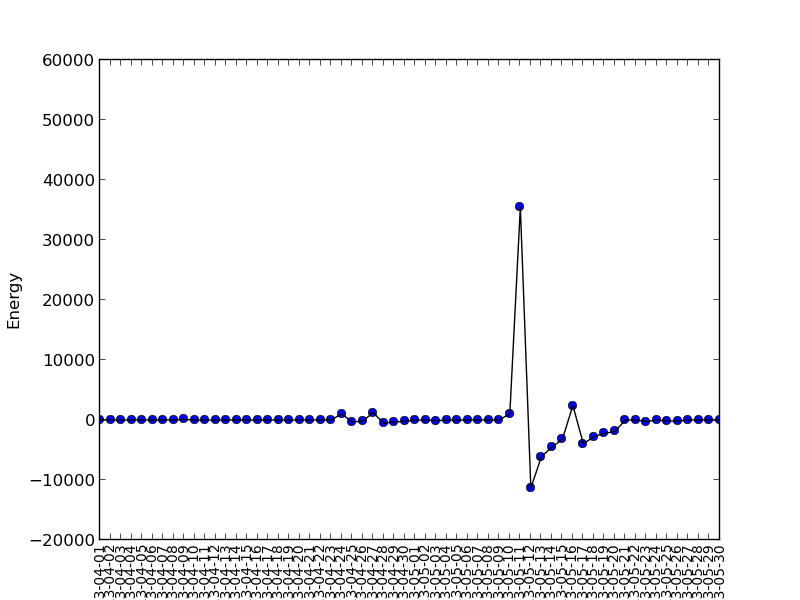
\includegraphics[width=0.45\textwidth]{格斗_energy.png}
}
\caption{词语“格斗”的nutrition值和energy值走势图}
\label{fig:7}
\end{figure}

\indent 从新兴词语到新兴话题的提炼,我们采用了聚类方法,将多个相关性较强的新兴词语(emerging term)聚成一个新兴话题(emerging topic)。Table 1是我们挖掘到的新浪微博中大社区中的一些新兴话题,或者说流行事件。4月20日发生的雅安地震,系统提取的关键词集合能够比较恰当地描述这个事件。5月5日的中大维纳斯歌手大赛决赛,我们提取到的关键词集合,也可以较好地表征这个事件(“冉彬学”是当晚的冠军)。美中不足的是,“维纳斯”这个关键字没有出现在这个关键词集合中。原因在于我们采用了聚类算法将新兴词语聚成一个新兴话题,因此,在同一个时间间隔中的一个词语只会出现在一个事件关键词集合中。这是一个较强的假设,如果在同一个时间间隔中爆发了两个不同的流行事件,并且该流行事件都包含有同一词语,那么,这个词语只会出现在其中一个事件关键词集合中,假如该词语对于表征这两个事件都非常重要,那么我们获得的其中一个关键词集合对特定事件的表征能力会差很多。\\
\indent 5月7日有一条微博在中大社区被大量转发,是一位中大的肿瘤学女博士(微博昵称为dr-where)上传了自己的本硕博自拍照,由于照片清新靓丽,一举扫荡了女博士在人们心目中大多是灭绝师太的印象(我们认为这是一种偏见),引来众多微博用户的围观,因此,成为了当天的流行事件。5月11日,格斗大赛的视频在微博中大社区被大量转发。当天,明星祝福维纳斯歌手大赛的视频也被大量转发,因此,这两个事件均成为当天的新兴事件。
\begin{table}[htbp]
\caption{\label{tab:test}微博流行事件}
\centering\begin{tabular}{|c|c|c|}
\hline
时间 & 事件关键词集合 & energy平均值 \\
\hline
4/20 & 雅安/四川/灾区/救援/祈祷/祈福/捐款/记者/生命/芦山 & 94,645 \\
\hline
5/5 & 冉彬学/10/直击/决赛/妹子/冠军/现场/期待/精彩 & 2,047 \\
\hline
5/7 & 本硕博/连读/where/dr/见识一下/女博士/逆袭/美女/男女 & 5,068 \\
\hline
5/11 & 格斗/自由/Din/师兄/第一节/一位/基裂/第一届/主页/更多/大赛 & 10,004 \\
\hline
\multirow{4}{1cm} {5/11} & 视频/维纳斯/11/沈佳宜/决赛/梦想/明星/感谢/祝福/球场/ & \multirow{4}{1cm} {14,662} \\
 & 风雨/不见不散/方大同/日晚/出炉/michelle/陳妍/金莎/终版/ & \\
 & 李易峰/痴狂/zTnvS1s/GBTers/千万种/珠海/林志炫/张芸京/ & \\
 & TerryLin/shane/PeggyHsu/许哲佩/曹轩/家林 & \\
\hline
\end{tabular}
\end{table}



\section{总结}
在这次项目中,大量数据的爬取和操作给我们带来了各种的挑战,但同时也让我们体现到与大数据做斗争的乐趣。这次的微博流行事件的爬取,依然存在着以下几个问题:
\begin{enumerate}
    \item 从term到topic的聚类过程仍然存在不令人满意的地方。某些term本来属于一个topic却在聚类后被分到不同的topic中。有些本来不属于同一个topic的term却被聚类为一组。
    \item topic中的term对事件的表征性不强。即使相关term组合起来的topic仍然难以表达一个特定的事件。
\end{enumerate}



\section{参考文献}
\begin{enumerate}[ {[}1{]} ]
\item Mario Cataldi, Luigi Di Caro and Claudio Schifanella. Emerging Topic Detection on Twitter based on Temporal and Social Terms Evaluation. In MDMKDD'10.
\item Brendan J. Frey* and Delbert Dueck. Clustering by Passing Messages Between Data Points. In science, 2007 - sciencemag.org.
\end{enumerate}


\end{document}
